\documentclass[11pt]{article}
\usepackage[margin=1in]{geometry}
\usepackage{amsmath,amssymb}
\usepackage{booktabs}
\usepackage{tikz}
\usetikzlibrary{arrows.meta,positioning}
\usepackage{parskip}
\usepackage[hidelinks]{hyperref}

\title{How the Housing Starts Nowcast Works\\[4pt]\large The math, as simply as possible}
\author{}
\date{November 2026}

\begin{document}
\maketitle

\section{The big idea}

A house can't be started until it has a building permit, and most permitted
homes start within a few months. So if we know \emph{how many} permits are
waiting and \emph{how long} each has been waiting, we can estimate how many
will start next month.

The model follows every permit through a two-stage pipeline:

\begin{center}
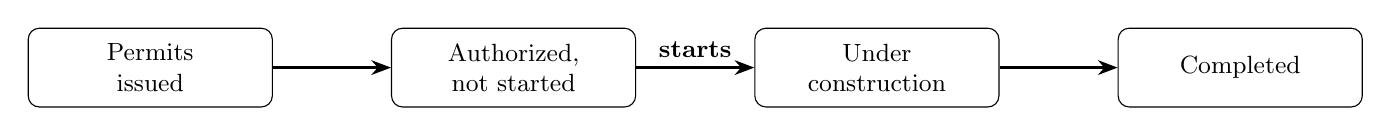
\begin{tikzpicture}[
  box/.style={draw, rounded corners, minimum width=3.1cm, minimum height=1cm, align=center, font=\small},
  arr/.style={-{Stealth[length=2.5mm]}, thick},
  node distance=1.5cm]
  \node[box] (p) {Permits\\issued};
  \node[box, right=of p] (ans) {Authorized,\\not started};
  \node[box, right=of ans] (uc) {Under\\construction};
  \node[box, right=of uc] (c) {Completed};
  \draw[arr] (p) -- (ans);
  \draw[arr] (ans) -- node[above, font=\small]{\textbf{starts}} (uc);
  \draw[arr] (uc) -- (c);
\end{tikzpicture}
\end{center}

The flow out of the first box is housing starts, which is the number we want
to forecast. There are two copies of the pipeline, one for single-family
(1-unit) homes and one for multifamily (2+ units) buildings, because
apartment buildings take much longer. The two results are added together at
the end.

\section{Step 1: Waiting-time shares become monthly ``start chances''}

The Census Survey of Construction reports how long permitted homes wait
before they start. For 2025 single-family homes:

\begin{center}
\begin{tabular}{lccccc}
\toprule
Months waited & 0 & 1 & 2 & 3 & 4+ \\
\midrule
Share of homes that start then & 37\% & 34\% & 12\% & 6\% & 11\% \\
\bottomrule
\end{tabular}
\end{center}

The model needs a slightly different number: the chance that a home
\emph{still waiting} at age $a$ starts this month. This is called the
\textbf{hazard}, $h_a$:
\[
  h_a \;=\; \frac{\text{share that start at age } a}{\text{share still waiting at age } a}.
\]

Worked through:
\begin{align*}
h_0 &= 0.37 / 1.00 = 0.37 \\
h_1 &= 0.34 / 0.63 = 0.54 \qquad (63\% \text{ were still waiting after month } 0)\\
h_2 &= 0.12 / 0.29 = 0.41 \\
h_3 &= 0.06 / 0.17 = 0.35
\end{align*}

\paragraph{The ``4+ months'' group.} This group has no end point, so the
model gives it one constant hazard $h$. If a home has a chance $h$ of
starting each month, its expected extra wait is $(1-h)/h$ months. The model
chooses $h$ so that the average wait across all homes matches the Census's
published 2025 average (1.4 months for single-family):
\[
  \underbrace{0(0.37) + 1(0.34) + 2(0.12) + 3(0.06)}_{=\,0.76}
  \;+\; 0.11\left(4 + \frac{1-h}{h}\right) \;=\; 1.4
  \quad\Longrightarrow\quad h \approx 0.355 .
\]

\paragraph{Wider buckets.} The construction-time data come in 3-month bins
(1--3 months, 4--6 months, \dots). For those, the model uses one hazard $p$
for all three months of the bin, chosen so the bin gets the right share:
\[
  S \cdot \bigl(1-(1-p)^{3}\bigr) = \text{bin share},
\]
where $S$ is the share still in the stage when the bin begins.

\section{Step 2: Not every permit becomes a start}

The Census timing shares only describe homes that \emph{do} eventually start.
In practice:
\begin{itemize}
  \item Multifamily: about \textbf{79\%} of permitted units start (some projects are
        dropped or re-permitted).
  \item Single-family: about \textbf{103\%}, because some homes are built in areas that
        don't issue permits.
\end{itemize}
Each month's permits are therefore scaled by a \textbf{conversion ratio}
\[
  c_t = \frac{\text{total starts over the previous 36 months}}{\text{total permits over the previous 36 months}},
\]
which uses only data from before month $t$, so the backtest never sees the
future.

\section{Step 3: Move everyone forward one month}

For each segment, the model keeps a list of how many units are waiting at each
age:
\[
  \mathbf{x}_t = \bigl(x_{t,0},\; x_{t,1},\; x_{t,2},\; \dots,\; x_{t,K}\bigr),
\]
where $x_{t,a}$ is the number of units that have been waiting $a$ months at
the end of month $t$, and the last slot holds everything ``$K$ or more''
months old. Each month does three things:

\begin{enumerate}
  \item \textbf{Starts.} Each age group sends its hazard share forward:
  \[
    \text{Starts}_t \;=\; \sum_{a} x_{t-1,a}\, h_a .
  \]
  \item \textbf{Survivors get one month older:}
  \[
    x_{t,a+1} = x_{t-1,a}\,(1-h_a).
  \]
  \item \textbf{New permits enter at age 0:}
  \[
    x_{t,0} = c_t \times \text{Permits}_t .
  \]
\end{enumerate}

The starts that leave stage 1 become the new arrivals in stage 2 (under
construction), and the same three rules apply there to produce completions.

\paragraph{Toy example.} Take 100 single-family permits with $c=1.03$, which
gives 103 effective units.
\begin{center}
\begin{tabular}{lccc}
\toprule
Month & Waiting at start of month & Hazard & Starts \\
\midrule
1 & 103.0 & $h_0 = 0.37$ & 38.1 \\
2 & 64.9  & $h_1 = 0.54$ & 35.0 \\
3 & 29.9  & $h_2 = 0.41$ & 12.4 \\
\bottomrule
\end{tabular}
\end{center}
Those starts are 37\%, 34\%, and 12\% of the 103 units, which are exactly
the Census shares. The hazards rebuild the original timing distribution.

\paragraph{Timing convention.} A permit issued in month $t$ can first start
in month $t+1$, using the Census ``same month'' share as its first-month
chance. In testing, this fit the data better than allowing same-month starts.

\section{Step 4: The nowcast}

The model runs this loop over the full permit history, through the last
published month (October 2026). That gives an estimate of how many units are
waiting at each age. November's starts are then simply
\[
  \widehat{\text{Starts}}_{\text{Nov}} \;=\; 12 \times \sum_{\text{segments}}\;\sum_{a} x_{\text{Oct},a}\, h_a .
\]
The factor of 12 converts the monthly count to a seasonally adjusted
annual rate (SAAR), the units Census uses. Every input is already published,
so no guess about November's permits is needed.

\begin{center}
\begin{tabular}{lr}
\toprule
Component & SAAR (thousands) \\
\midrule
From October's permits (newest cohort) & 418 \\
From older permits still waiting & 856 \\
\midrule
\textbf{November 2026 nowcast} & \textbf{1{,}274} \\
\addlinespace
\quad Single-family / Multifamily & 857 / 417 \\
\quad vs.\ October 2026 actual (1{,}309) & $-35$ \;($-2.7\%$) \\
\quad vs.\ November 2025 actual (1{,}319) & $-45$ \;($-3.4\%$) \\
\bottomrule
\end{tabular}
\end{center}

\section{How well it fits}

Over the 24 months to October 2026, the model's monthly starts miss the
actual figure by an average of \textbf{62k SAAR} (mean absolute error). The
correlation with actual starts is \textbf{0.45}, and the average bias is
about $-9$k (essentially unbiased).

\section{Shortfalls of the model}

The model is best read as a trend-level estimate, not a precise forecast of
one month. First, its timing assumptions are fixed. Every hazard is calibrated
to a single year (2025) of national Census averages, and the permit-to-start
conversion rate is a trailing 36-month ratio. Both are slow to react when
builders speed up, slow down, or cancel projects at turning points, which is
exactly when a nowcast matters most. Second, the pipeline is not sized
exactly right. The modeled stock of permitted-but-not-started units runs about
16\% above the Census figure, and the under-construction stock about 10\%
below. That points to remaining errors in the conversion and timing
assumptions. The timing convention also pushes the Census ``same month''
starts back by one month. Third, it ignores everything outside the permit
pipeline. There are only two segments (single- vs.\ multifamily), with no
regional detail, and no inputs for weather, mortgage rates, builder
sentiment, or one-off large apartment projects, which drive much of the
month-to-month noise in starts. Fourth, the evaluation flatters the model. It
is tested on today's revised data rather than the first-print figures
available in real time, over only 24 months. Over that window, its error
(62k SAAR) is no better than a simple regression on lagged permits, starts,
and backlog (also 62k). Finally, a 62k miss is small against the Census's own
90\% confidence interval for the monthly change in starts (roughly
$\pm$10--14\%), but it still means a single-month print anywhere from about
1{,}210k to 1{,}340k is consistent with the 1{,}274k nowcast. The model
reports no formal uncertainty band of its own.

\end{document}
